\documentclass[A4paper, 12pt]{article}
\usepackage{fancyhdr}
\usepackage{graphicx}
\usepackage{booktabs}
\usepackage{pdfpages}
\usepackage[UTF8]{ctex}
\pagestyle{fancy}
\lhead{Vulcano 2.0:  全新开端}
\rhead{v2.03 CHI}
\cfoot{\thepage}
\renewcommand{\headrulewidth}{0.4pt}
\renewcommand{\footrulewidth}{0.4pt}
\begin{document}
\title{Vulcano 2.0: A New Beginning}
\author{The Vulcano Team}
\date{\today}
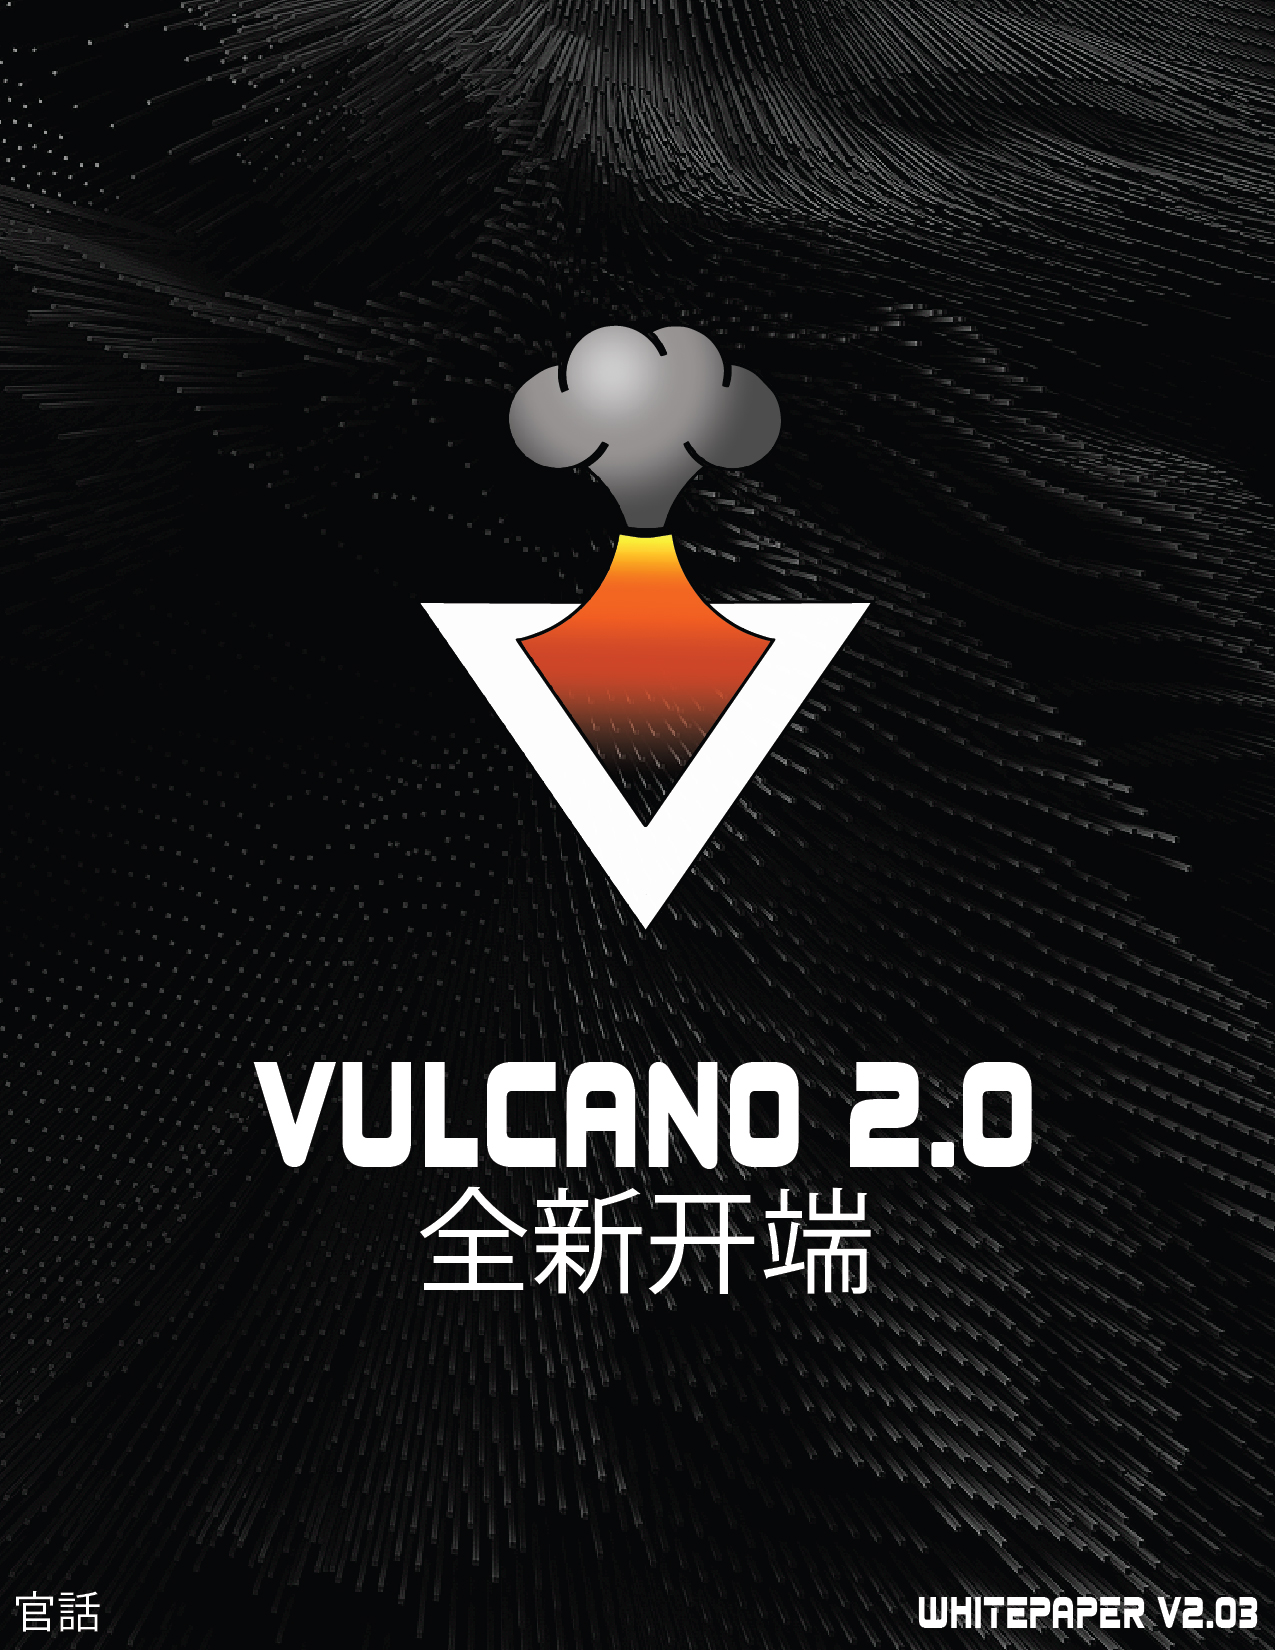
\includepdf[pages=1]{COVER-CHI.jpg}
\newpage
\tableofcontents
\newpage
\section{介绍}

Vulcano(股票代码:   VULC)是一种面向网络社区的网络货币,最初是在2017年底由一个全新的开发团队创建的。   最初,它被认为仅仅是一款“高价网络货币”,年回报率为950\%。  然而,由于最初开发团队的一些错误,实际率接近320000\%。   这一点一直没有被注意到,直到某个社区成员通过研究创始街区1的区块链来计算这个有效率。  一旦这一基本弱点暴露出来,新的 Vulcano 团队,包括社区成员,一起通过一个完整的重建和开发一个真正的使用案例,在技术和设计理念层面上挽救了 Vulcano 项目。   这本白皮书提出了一个全面升级的 Vulcano 策略和重新升级的网络货币,作为资助地热勘查和研究的手段。 

我们不只是简单地解决与 Vulcano 的比率问题,而是选择将网络货币完全升级到一个新的代码库。   为了使 Vulcano 核心现代化,Vulcano 团队决定将堡垒作为代码基础。   堡垒是建立在 PIVX 上的,它本身是建立在流行的 DASH 加密算法之上的。  这个关键的决定将使我们有能力实现主节点的功能和管理,并最终允许硬件节点的集成,以支持 Vulcano 生态系统。  这样做,我们将创建一个更为分散的管理体系,网络货币定位系统和网络安全系统。

本文还将通过建立 Vulcano 基金会,为 Vulcano 的合法化制定未来的计划。这是一个计划在美国的 501(C)3 非盈利实体,它将允许 Vulcano 以一种成熟的方式成长为自己的公司,并开始与其他商界建立联系并进行谈判。这一点尤其重要,因为 Vulcano 的长期使用案例要求通过下面解释的研究机制来获取知识产权的投资组合。  通过在全球各地的大学和研究机构的资助下,创建一个知识产权投资组合。   Vulcano 基金会将使我们能够充分利用这一知识产权。这是一个绝对关键的步骤,它将允许分散的 Vulcano 项目与商业界和学术界互联。 

本文还将制定计划管理费用所占的百分比,这将直接资助地热研究,以提高科学研究和获取知识产权,为 Vulcano 基金会的未来发展提供更多基金,并提供额外拨款。 

您在本文中找不到的是对 Vulcano 区块链未来的荒谬和未经证实的承诺。  Vulcano 力争创新和发展,不做不能兑现的承诺,而是致力于研究和促进技术发展。本文所提到的所有区块链技术已经被证明并将在适当的时候被激活。   我们相信,现在是加密社区开始行动的时候了,这是与他们带来的商业潜力相一致的,而不需要区块链技术的荒诞说法来建立一个使用现有技术的商业案例。  开发者、团队领导和社区本身必须明白,为了被更广泛的商业和学术社区所接受,我们必须愿意在一定程度上遵守他们的规则。在区块链技术被开发、测试或计划之前,在提出关于未被证实的区块链技术的想法之前,先充分利用我们所拥有的知识。虽然区块链技术在未来可能会为 Vulcano 带来新的进展,但它的发布不会随着数月的宣传和营销而到来,但一旦它已经被开发出来了,就只有它会被提及了。  我们相信,这种“潜艇”发展方式对于货币来说是最好的,因为它限制了投机性投资,并为未来的平台建设奠定了坚实的基础。 

我们的目标是把 Vulcano 变成未来可持续发展研究的主要资金来源之一,并最终建立一个围绕这项技术的商业生态系统。

\section{致谢}
如果没有比特币、Peer-coin、黑币、Talkcoin、DASH、PIVX 以及最重要的 Bulwark 团队的前期工作,Vulcano 就不可能做到这些。  因为 Vulcano 的新化身是一个改良的 Bulwark 分岔,所以我们有几个部分直接从他们的白皮书中借来。这些我们将包括但不会从现有的代码库中进行修改。我们,Vulcano 团队,认为将这些章节包含在 Bulwark 文件中,而不是重写它们,假装它们是完全原创的,是更为透明的。  然而更重要的是,作为一个社区,我们要开发适用于更广泛世界的实体用例和业务结构,必须保护和维护未来的数字加密货币背后的开源精神。普遍说来,人类受益于信息共享,我们为贡献这一不断增长的知识而感到自豪。        正是本着同样的精神,我们将给为 Vulcano 生态系统做出贡献的国家提供通过 Vulcano 基金会资助的技术。

\section{数字加密货币的简介}
虽然分布式分类账技术的建议可以追溯到20世纪80年代末,但直到一篇题为“比特币”的论文在一个晦涩难懂的密码学公告板上发表,  一个以 Satoshi Nakamoto 的笔名为基础的对等电子现金系统,一个真正的区块链才诞生了。区块链通过时间戳交易来工作,并将它们锁定成“块”,这些块通过各种方法验证,从而不会被篡改。比特币和许多其他数字加密货币技术在“工作证明”的基础上运行,这意味着他们计算能力是他们网络中稀缺资源的来源。

然而,由于 Vulcano 关注的是可持续性和在能源领域的研究,这种不可持续的方法与我们努力提高可持续性的做法背道而驰。因此,我们已选择以“股份证明”为基础运作。于此,网络资源稀缺性是代币本身。  此外,随着升级后的 Vulcano 推出30天后,我们发布此白皮书,我们也将拥有主节点,这是一种更先进的“股份证明”版本,在该版本中,世界各地的计算机维护网络,而且为此,承担一些简单的计算负载。就目前而言,这个计算负载几乎不比简单的赌注钱包的操作更大,但是,我们希望将来使用这个网络来为可再生能源产业进行分布式计算,以用于计算化学和物理问题。这是 Vulcano 长期规划的重要补充,如地球物理学和地热部门。在研究型大学中,通常不像其他更为炫耀的领域那样有充足的资金,因此在大计算机上运行周期性的时间来运行他们的模拟变得更加困难。 

此外,从消费者的角度来看,在90秒的区块时间、主节点共识和交易锁定、可控和稳定的排放时间表和生态友好的股票行情中,Vulcano 渴望成为真正快速的和功能性的数字加密货币,从而对世界产生真正的影响,成为消费者和数字加密货币爱好者的一个强有力的选择。

\section{新 Vulcano}
\subsection{新 Vulcano 区块链的详情}

\begin{table}[h]
\centering
\begin{tabular}{@{}ll@{}}
\toprule
股票行情 & VULC \\ \midrule
算法 & NIST5 \\
RPC 端口 & 62541 \\
P2P 端口 & 62543 \\
区块间距 & 90秒 \\
的难度算法 & Dark Gravity Wave v3.0 \\
区块大小 & 1MB \\
挖掘/到期成熟 & 块(100分钟) \\
确认 & 6块(9分钟) \\
循环周期(1年) & 246,194,250 \\
循环周期(5年) & 421,126,225 \\
PoW 周期 & nHeight: 60 \\
PoS 周期 & nHeight: 61 \\
协议支持 & IPV4, IPV6, TOR \\
PoS & Blackcoin v3.0 PoS \\ \bottomrule
\end{tabular}
\end{table}

\subsection{	让社区保持 团结}
Vulcano 最初被设想为一款社区网络货币,这是我们全心全意相信的想法。作为一款社区网络货币,我们知道服务于该项目发展的最佳方式是服务于我们所欠的社区。我们将继续努力、比赛等以社区为基础的活动。我们还将促进对 Vulcano 生态系统的局限性的讨论和探索。  在所有论坛中,我们将对新来者、用户和其他数字加密货币社区的骚扰保持零容忍政策。  Vulcano 认为,在数字加密货币世界中有足够的空间,我们可以并且应该努力合作和协作,而不是对其他项目进行拆台。  虽然我们坚持认为,在不同的数字加密货币平台之间存在着一定程度的良好的本质竞争,但我们希望所有的互动都是积极的。 

\subsection{建设业务的能力}
在写作的时候,已经出现了利用相似的技术基础的数字加密货币的汇集。  虽然底层技术是可靠的,但经常对它们的规格和区块链参数的更深入的检查揭示了不公平的做法。  在其他情况下,技术实施是很差的,但社区没有足够的信息来确定这些问题,并参与了根本不健全的项目。

不幸的是,原来的 Vulcano 很容易落入这个范畴,这是新 Vulcano 团队全面扭转该项目的主要原因之一。  我们相信,数字加密货币应该有真正的商业应用,这种技术不应该只用于在市场了解真正发生什么之前采取行动的少数持有者创造投机收入。  我们经常看到开发商开发出一款不好的网络货币,用华丽的广告来宣传它,然后在作为持币人离开社区时放弃这个项目。   这就是为什么我们相信透明度和问责制,并将建立必要的商业基础来做真正的业务,包括数字加密和非加密两种。 

因此,我们将建立几个正式的商业组织,以促进这些互动。  首先最重要的是我们将建立的 501(c)3 非营利组织,目的是将资金引导到地热和其他地球科学研究计划。  该组织将负责维护任何知识产权和商标标志。 

也将有一系列LLCs为世界各地的地方要求而建立。许多数字加密货币交换要求本地业务 实体,并且可以通过建立 LLCs 网络来提供。  这个网络将给予 Vulcano 基金会和 Vulcano 社区在世界任何地方开展业务的能力,而不丧失适应当地需求和法律要求的能力。

\subsection{维护 社区}
VULC 社区是项目长期成功背后的最重要因素,它们对网络货币未来的影响和关键领域的技术发展是至关重要的。由于我们的首要目的是通过几乎不受限制的地热发电机制来推进可持续性研究,我们已经制定了行动计划,为在这些领域工作的研究人员提供资金。 

因此,在我们第一年结束时,在第172801区块,我们打算激活网络上的预算爆发块。  这些爆发块,按月支付,将使社区对研究发挥有意义的控制。包括 Vulcano 资金,品牌发展的存在,以及社区事务。从启动开始延迟该系统大约六个月将给我们时间来开发一个积极的用户体验所必需的基础框架,并允许系统从代币发散率的变化中稳定下来,从320000\%减少到某个更合理的程度。

此外,将有10\%的管理结构添加到所有的区块奖励,将透明地并可追溯地用于资助地热研究。随着这个继续,除了那些我们通过自己的努力选择的,我们还将利用一个多阶段的过程来创造和提交建议。  为了一个建议被接受,选择过程中的每一步都需要充分完成。   由于我们相信智慧和知识可以来自于各种各样的地方,我们鼓励 Vulcano 社区对围绕地热能源的技术进行构思。  这些建议和想法将汇集在一起,并可以在学术层面上对其更深入地探索之前由其他社区进行投票和讨论。  我们希望 Vulcano 社区能够吸引来自世界各地的地热专家为这一构想进程做出贡献。

\subsection{Vulcano 发散 率}
以下是 Vulcano 区块链的区块奖励和发散率。
\begin{table}[h]
\centering
\begin{tabular}{@{}ccccc@{}}
\toprule
月份 & 区块号码 & 区块奖励 & 发散的 & 总计 \\ \midrule
0 & 0-1 & 95,000,000 & 95,000,000 & 95,000,000 \\
1-6 & 2 to 172800 & 500 & 86,396,500 & 181,396,500 \\
7-12 & 172801 to 345600 & 375 & 64,797,750 & 246,194,250 \\
13-18 & 345601 to 518400 & 281.25 & 48,598,313 & 294,792,563 \\
19-24 & 518401 to 691200 & 210.94 & 36,448,734 & 331,241,297 \\
25-30 & 691201 to 864000 & 158.20 & 27,336,551 & 358,577,848 \\
31-36 & 864001 to 1036800 & 118.65 & 20,502,413 & 379,080,261 \\
37-42 & 1036801 to 1209600 & 88.99 & 15,376,810 & 394,457,071 \\
43-48 & 1209601 to 1382400 & 66.74 & 11,532,607 & 405,989,678 \\
49-54 & 1382401 to 1555200 & 50.06 & 8,649,456 & 414,639,133 \\
55-60 & 1555201 to 1728000 & 37.54 & 6,487,092 & 421,126,225 \\
61+ & 1728001 到无穷大 & 18.77 & 继续 & 继续 \\ \bottomrule
\end{tabular}
\end{table}

\subsection{	努力战胜 集中化}
目前存在的区块链生态系统有的几个问题。  这些问题,虽然它们存在于不同的领域中,但都可以被描述为过度集中的一种或另一种方式。 

必须消除的第一类集中是绝大多数的代币或网络货币掌握在投机者的手中。这导致了完全不合理的价格波动,因为各种各样的行动者试图操纵市场,而不知情的投机者正在迅速地寻找下一个“圆月”买入和卖出仓位。   虽然这对实际发展几乎没有影响,但它在社区内形成了一种态度,即当它们完全没有联系时,价格波动在某种程度上决定或反映了项目的基本健康状况。  投机者手中的集中化问题导致波动性和高度风险性。             我们的目标之一是尽可能最大限度地管理这个方面。

第二种类型的集中化是指地理上集中化的虚拟专用服务器,在这些服务器上通常配置主节点。   通过提供廉价的主节点托管服务,社区有一种倾向在单个节点上部署大量节点。服务提供商,意味着一个不可预见的事件可以抹去网络的很大一部分,从而导致漏洞。 

解决这个过度集中的双重问题的一个方法是 Vulcano 研究生态系统。由于 Vulcano 基金会资助地热领域的研究,预计它将获得一个知识产权的组合。以极低的成本提供给将同意主办 Vulcano 硬件节点的任何机构或国家是我们的计划。2 这样,这些机构将有一组技术工具作为他们自己技术的构建块,用于在他们自己的系统上或在 Vulcano 硬件节点上部署主节点的简单成本。    这将极大地增加 Vulcano 主节点的地理分布,同时也减少了在社区中漂浮的代币数量,而且可用于推测。

我们还认为,Vulcano 代币尽可能广泛地分发是很重要的。事实上,我们相信,大多数较小的数字加密货币项目都有很大比例的代币在少数持有者手中,这给项目带来了某种程度的集中化危险。  因此,我们打算在未来推出计划,以激励去中心化和大钱包的分散,并奖励那些拥有少量主节点的人。这将在以后讨论。

由于 Vulcano 团队是开源开发的有力支持者,我们希望在尽可能多的领域保持这种近乎开源的商业模式。当然,所有的源代码都随时可供检查,但是我们也希望尽可能便宜地提供一整套知识产权。

\section{Vulcano 特色}
\subsection {主节点}
主节点合起来是一个分散的计算机网络,为 Vulcano 网络服务。  他们执行重要的网络功能,并获得部分区块奖励。除了提供这些基本的网络功能外,他们还通过稳定的网络货币供应、处理交易操作和保护网络安全。主节点需要50,000 VULC和适度的技术知识才能运行。任何控制50,000 VULC的钱包都可以建立一个主节点。

Vulcano团队有引入各种类型节点的长期计划,这些节点将根据它们对有用的计算网络的贡献给予奖励。这样,可以回避“工作证明”的挑战,因为正在进行的计算不是保护网络安全的任意计算,而是有助于可持续性科学进步的功能计算。  随着事态的进一步发展,我们将会发布关于这项提议的更多信息。

\subsection{混淆/网络货币 混合}
由于新的 Vulcano 核心代码是基于 Bulwark 的,它还具有混淆功能,这是通过主节点网络以分散的方式实现的。这在交易中提供了额外的隐私层。虽然不是完全匿名的,但通过节点混合进行混淆远优于标准比特币交易。   例如,所有比特币交易都是透明的,可以很容易地在整个区块链跟踪。  对于 Vulcano 来说,一个邪恶的行为者需要控制至少50\%的操作主节点,才有超过0.5\%的机会去匿名一个与8轮混淆混在一起的交易。  这一重要功能为选择隐藏交易的VULC用户提供了非常高的匿名性。   虽然与Vulcano项目的最终用例没有密切联系,但它提供了一定程度的消费者可用性,相对于其他处于密码阶段的项目来说,这提高了它的价值。

\subsection{SwiftTX}
SwiftTX为主节点提供了交易的锁定和一致授权。当交易提交到网络时,一组主节点将验证交易。  如果这些主节点对交易的有效性达成共识,它将被锁定,以便以后引入区块链,与传统系统相比,交易速度大大提高(比如比特币10分钟的阻塞时间,有多个限制)。SwiftTX使得在用相同的输入挖掘网络上的块之前,可以进行多个事务。  该系统基于 Dashs InstantSend。

\subsection{Sporks}
新的Vulcano网络采用了在Bulwark引入的多相叉形机构,被称为“sporking”。  这将使VULC网络能够实现新的功能,同时最大限度地减少部署过程中出现意外网络分叉的机会。  Spork更改可以通过网络部署,并且可以根据需要打开和关闭,而无需更新节点软件。   这个功能非常有用,允许网络对安全漏洞做出快速反应,而不需要单个用户的输入来手动更新他们的钱包代码。

\subsection{TOR和IPV6主节点}
Vulcano 将允许用户从TOR地址或IPV6地址运行他们的完整节点或主节点。  我们一直致力于添加完整的TOR节点,以增强TOR网络本身,以及在仅TOR模式下运行的 Bulwark 用户体验。TOR MAS - ternode支持的一个独特功能是能够将您的主节点作为TOR隐藏服务来操作。TOR节点使具有稳定互联网连接的用户能够在其家庭网络之外操作主节点,而不会暴露其位置或暴露其家庭网络可能受到攻击或危害的隐私影响。

\section{未来计划}
\subsection{Vulcano安全硬件节点}
Vulcano团队的关键成员目前正在与高端消费电子产品的专业制造商合作,开发安全的硬件节点,这些节点可以在全球部署,以分散网络和提高安全性。  用户将能够将其连接到他们的家庭网络,并使用Web UI进行配置。我们打算使用TOR隐藏服务为那些拥有稳定互联网连接的用户轻松设置完全隐私化主节点(或完全节点)的功能。

本着权力下放的精神,社区可以获得所有源代码进行家庭组装,但也可以通过现成的模式获得。这些节点也将是由Vulcano Foundation发布,旨在通过部署静态节点来增加地理分布和网络货币锁定。

\subsection{Vulcano商店}
当务之急是为Vulcano创建一个真实的用例。这方面的第一个例子是在Vulcano区块链经营的数字产品市场。虽然这最初是针对社区以外的数字商品,如蒸汽代码和礼品卡,但它计划扩展成为一个基于Vulcano的点对点市场。

\subsection{电报与不协调的机器人}
每个区块链项目的灵魂都是社区,服务社区的最大方式之一就是给他们一种交流和使用令牌的方式。Vulcano团队将资助为各种聊天服务创建机器人,这将使人们能够轻松地与世界其他地方分享他们的虚拟世界。  通过促进Vulcano的这种自由流动,我们可以提高效用,同时也可以吸引和发展社区。

\section{结论}
Vulcano 离几个月前首次发现关键弱点的情形还有很长一段路要走。我们正在对新的 Vulcano 区块链进行测试,其功能正在扩展,并且已经做了大量工作来修复已经使项目和社区瘫痪数月的问题。我们很高兴宣布这些变化和更新,也很高兴公布我们的长期计划。  这份白皮书将成为一份活的文档,我们期待着提供持续的更新。
\newpage
\section{Changelog}

\begin{table}[h]
\centering
\begin{tabular}{@{}ccccc@{}}
\toprule
版 & 日期 & 说明 \\ \midrule
v2.02 & August 3rd, 2018 & 首先是中文翻译 \\
 \bottomrule
\end{tabular}
\end{table}

\end{document}
